\documentclass[14pt]{extbook}
\usepackage{multicol, enumerate, enumitem, hyperref, color, soul, setspace, parskip, fancyhdr} %General Packages
\usepackage{amssymb, amsthm, amsmath, latexsym, units, mathtools} %Math Packages
\everymath{\displaystyle} %All math in Display Style
% Packages with additional options
\usepackage[headsep=0.5cm,headheight=12pt, left=1 in,right= 1 in,top= 1 in,bottom= 1 in]{geometry}
\usepackage[usenames,dvipsnames]{xcolor}
\usepackage{dashrule}  % Package to use the command below to create lines between items
\newcommand{\litem}[1]{\item#1\hspace*{-1cm}\rule{\textwidth}{0.4pt}}
\pagestyle{fancy}
\lhead{Progress Quiz 9}
\chead{}
\rhead{Version B}
\lfoot{9541-5764}
\cfoot{}
\rfoot{Summer C 2021}
\begin{document}

\begin{enumerate}
\litem{
Solve the quadratic equation below. Then, choose the intervals that the solutions $x_1$ and $x_2$ belong to, with $x_1 \leq x_2$.\[ 25x^{2} +75 x + 54 = 0 \]\begin{enumerate}[label=\Alph*.]
\item \( x_1 \in [-1.86, -1.47] \text{ and } x_2 \in [-1.31, -1.15] \)
\item \( x_1 \in [-46.12, -44.27] \text{ and } x_2 \in [-30.08, -29.85] \)
\item \( x_1 \in [-2.51, -2.32] \text{ and } x_2 \in [-1.13, -0.83] \)
\item \( x_1 \in [-5.87, -4.97] \text{ and } x_2 \in [-0.5, -0.33] \)
\item \( x_1 \in [-10.18, -7.05] \text{ and } x_2 \in [-0.31, -0.04] \)

\end{enumerate} }
\litem{
Write the equation of the graph presented below in the form $f(x)=ax^2+bx+c$, assuming  $a=1$ or $a=-1$. Then, choose the intervals that $a, b,$ and $c$ belong to.
\begin{center}
    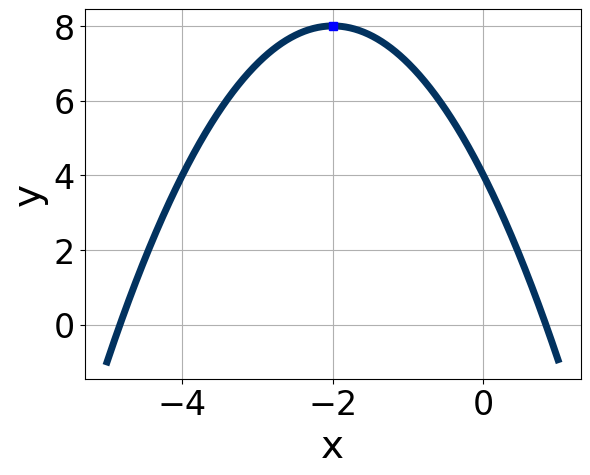
\includegraphics[width=0.5\textwidth]{../Figures/quadraticGraphToEquationB.png}
\end{center}
\begin{enumerate}[label=\Alph*.]
\item \( a \in [-2, 0], \hspace*{5mm} b \in [3, 8], \text{ and } \hspace*{5mm} c \in [4, 5] \)
\item \( a \in [-2, 0], \hspace*{5mm} b \in [3, 8], \text{ and } \hspace*{5mm} c \in [-12, -10] \)
\item \( a \in [-2, 0], \hspace*{5mm} b \in [-4, -1], \text{ and } \hspace*{5mm} c \in [4, 5] \)
\item \( a \in [0, 2], \hspace*{5mm} b \in [-4, -1], \text{ and } \hspace*{5mm} c \in [9, 14] \)
\item \( a \in [0, 2], \hspace*{5mm} b \in [3, 8], \text{ and } \hspace*{5mm} c \in [9, 14] \)

\end{enumerate} }
\litem{
Graph the equation below.\[ f(x) = -(x+1)^2 + 14 \]\begin{enumerate}[label=\Alph*.]
\begin{multicols}{2}\item 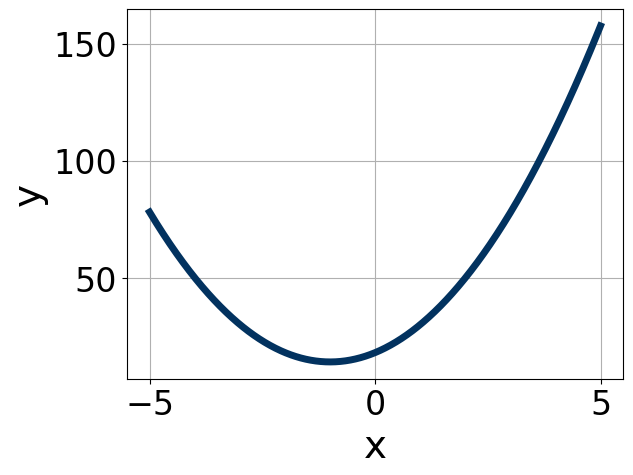
\includegraphics[width = 0.3\textwidth]{../Figures/quadraticEquationToGraphCopyAB.png}\item 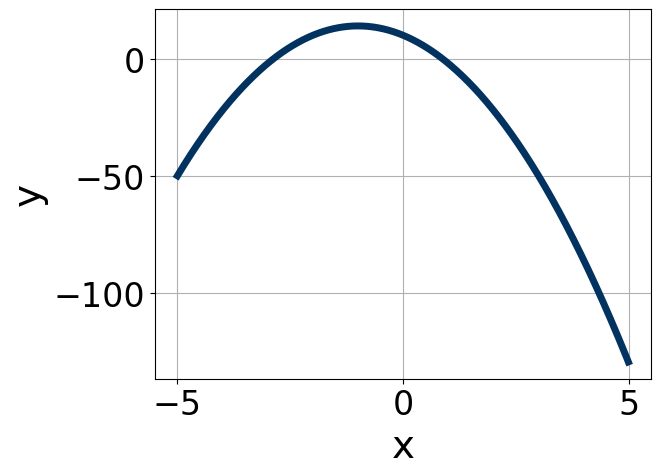
\includegraphics[width = 0.3\textwidth]{../Figures/quadraticEquationToGraphCopyBB.png}\item 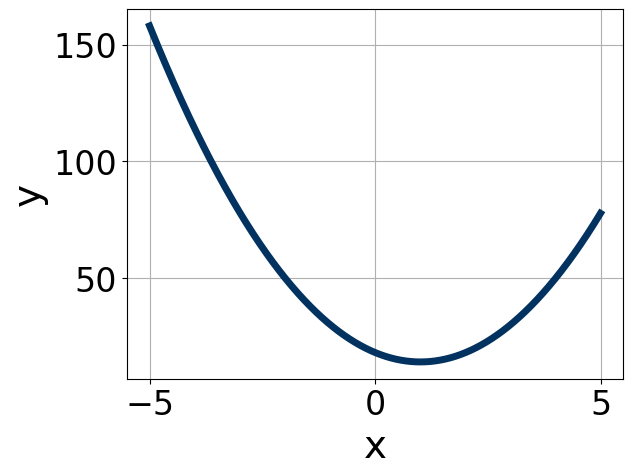
\includegraphics[width = 0.3\textwidth]{../Figures/quadraticEquationToGraphCopyCB.png}\item 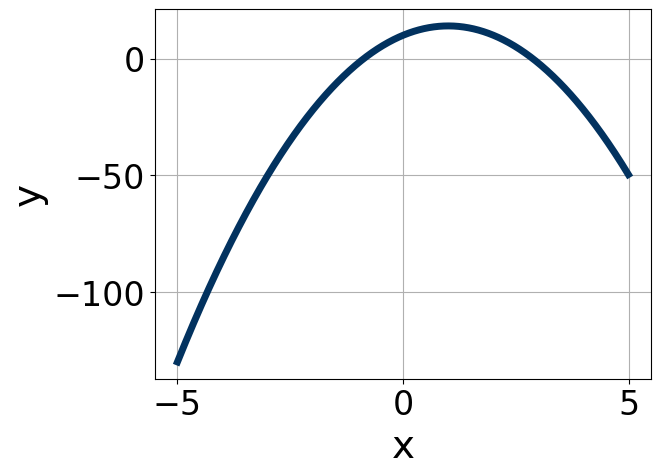
\includegraphics[width = 0.3\textwidth]{../Figures/quadraticEquationToGraphCopyDB.png}\end{multicols}\item None of the above.
\end{enumerate} }
\litem{
Graph the equation below.\[ f(x) = -(x+1)^2 + 12 \]\begin{enumerate}[label=\Alph*.]
\begin{multicols}{2}\item 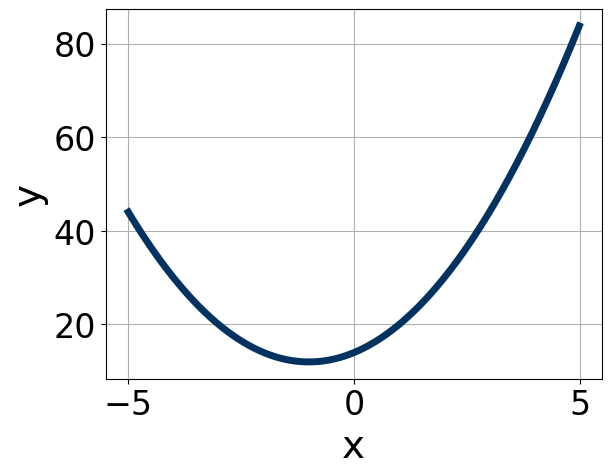
\includegraphics[width = 0.3\textwidth]{../Figures/quadraticEquationToGraphAB.png}\item 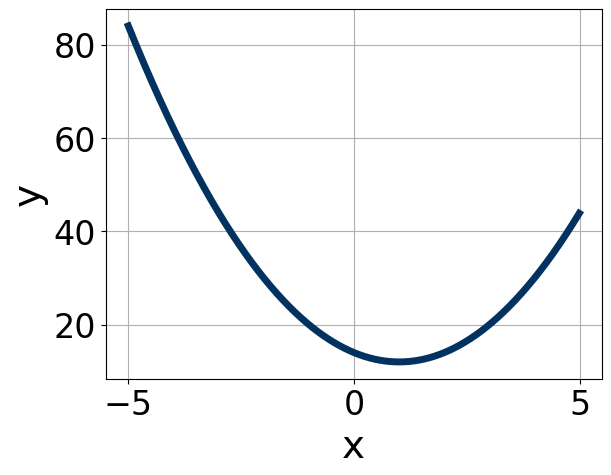
\includegraphics[width = 0.3\textwidth]{../Figures/quadraticEquationToGraphBB.png}\item 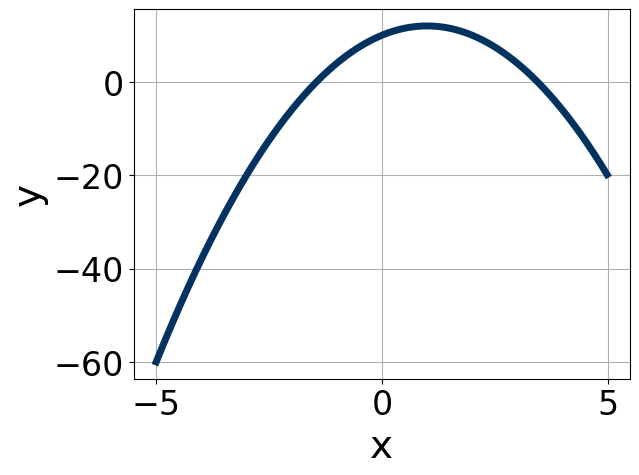
\includegraphics[width = 0.3\textwidth]{../Figures/quadraticEquationToGraphCB.png}\item 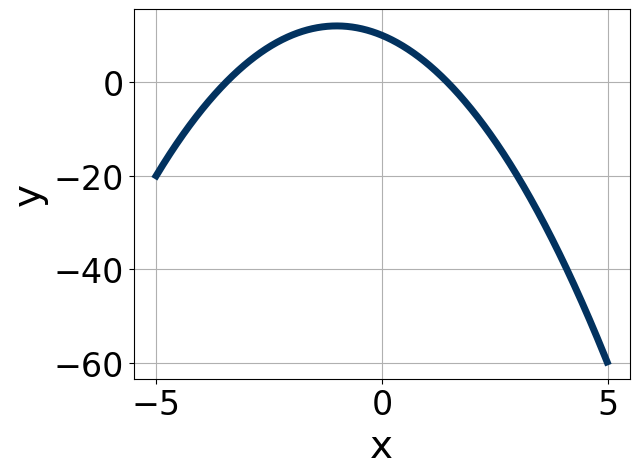
\includegraphics[width = 0.3\textwidth]{../Figures/quadraticEquationToGraphDB.png}\end{multicols}\item None of the above.
\end{enumerate} }
\litem{
Solve the quadratic equation below. Then, choose the intervals that the solutions $x_1$ and $x_2$ belong to, with $x_1 \leq x_2$.\[ 25x^{2} +50 x + 24 = 0 \]\begin{enumerate}[label=\Alph*.]
\item \( x_1 \in [-2.76, -1.62] \text{ and } x_2 \in [-0.44, -0.18] \)
\item \( x_1 \in [-30.33, -29.48] \text{ and } x_2 \in [-20.15, -19.54] \)
\item \( x_1 \in [-1.53, -0.44] \text{ and } x_2 \in [-1.02, -0.8] \)
\item \( x_1 \in [-6.4, -5.95] \text{ and } x_2 \in [-0.27, 0.26] \)
\item \( x_1 \in [-2.06, -1.47] \text{ and } x_2 \in [-0.79, -0.45] \)

\end{enumerate} }
\litem{
Solve the quadratic equation below. Then, choose the intervals that the solutions belong to, with $x_1 \leq x_2$ (if they exist).\[ -19x^{2} -14 x + 9 = 0 \]\begin{enumerate}[label=\Alph*.]
\item \( x_1 \in [-1.79, -0.99] \text{ and } x_2 \in [-0.31, 0.65] \)
\item \( x_1 \in [-30.36, -29.59] \text{ and } x_2 \in [29.26, 30.14] \)
\item \( x_1 \in [-8.31, -6.86] \text{ and } x_2 \in [21.46, 22.28] \)
\item \( x_1 \in [-1.06, 0.8] \text{ and } x_2 \in [0.92, 1.45] \)
\item \( \text{There are no Real solutions.} \)

\end{enumerate} }
\litem{
Write the equation of the graph presented below in the form $f(x)=ax^2+bx+c$, assuming  $a=1$ or $a=-1$. Then, choose the intervals that $a, b,$ and $c$ belong to.
\begin{center}
    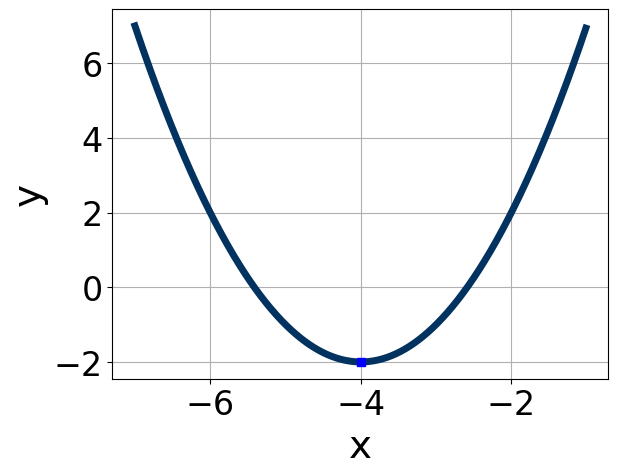
\includegraphics[width=0.5\textwidth]{../Figures/quadraticGraphToEquationCopyB.png}
\end{center}
\begin{enumerate}[label=\Alph*.]
\item \( a \in [-2.5, 0.6], \hspace*{5mm} b \in [-9, -7], \text{ and } \hspace*{5mm} c \in [-24, -15] \)
\item \( a \in [-2.5, 0.6], \hspace*{5mm} b \in [5, 12], \text{ and } \hspace*{5mm} c \in [-24, -15] \)
\item \( a \in [0.9, 1.5], \hspace*{5mm} b \in [-9, -7], \text{ and } \hspace*{5mm} c \in [13, 16] \)
\item \( a \in [0.9, 1.5], \hspace*{5mm} b \in [-9, -7], \text{ and } \hspace*{5mm} c \in [16, 22] \)
\item \( a \in [0.9, 1.5], \hspace*{5mm} b \in [5, 12], \text{ and } \hspace*{5mm} c \in [13, 16] \)

\end{enumerate} }
\litem{
Factor the quadratic below. Then, choose the intervals that contain the constants in the form $(ax+b)(cx+d); b \leq d.$\[ 24x^{2} -10 x -25 \]\begin{enumerate}[label=\Alph*.]
\item \( a \in [1.04, 2.41], \hspace*{5mm} b \in [-10, 0], \hspace*{5mm} c \in [10.5, 16.1], \text{ and } \hspace*{5mm} d \in [1, 9] \)
\item \( a \in [2.66, 5.06], \hspace*{5mm} b \in [-10, 0], \hspace*{5mm} c \in [5.6, 7.2], \text{ and } \hspace*{5mm} d \in [1, 9] \)
\item \( a \in [0.71, 1.26], \hspace*{5mm} b \in [-32, -28], \hspace*{5mm} c \in [-0.9, 2.2], \text{ and } \hspace*{5mm} d \in [20, 28] \)
\item \( a \in [6.55, 8.23], \hspace*{5mm} b \in [-10, 0], \hspace*{5mm} c \in [1.4, 4.5], \text{ and } \hspace*{5mm} d \in [1, 9] \)
\item \( \text{None of the above.} \)

\end{enumerate} }
\litem{
Factor the quadratic below. Then, choose the intervals that contain the constants in the form $(ax+b)(cx+d); b \leq d.$\[ 36x^{2} -60 x + 25 \]\begin{enumerate}[label=\Alph*.]
\item \( a \in [-2.7, 2.9], \hspace*{5mm} b \in [-31, -21], \hspace*{5mm} c \in [0.57, 1.73], \text{ and } \hspace*{5mm} d \in [-34, -27] \)
\item \( a \in [2.2, 5], \hspace*{5mm} b \in [-12, -3], \hspace*{5mm} c \in [11.82, 13.04], \text{ and } \hspace*{5mm} d \in [-5, -4] \)
\item \( a \in [5.7, 6.1], \hspace*{5mm} b \in [-12, -3], \hspace*{5mm} c \in [5.25, 6.79], \text{ and } \hspace*{5mm} d \in [-5, -4] \)
\item \( a \in [16.7, 20.6], \hspace*{5mm} b \in [-12, -3], \hspace*{5mm} c \in [1.01, 3.29], \text{ and } \hspace*{5mm} d \in [-5, -4] \)
\item \( \text{None of the above.} \)

\end{enumerate} }
\litem{
Solve the quadratic equation below. Then, choose the intervals that the solutions belong to, with $x_1 \leq x_2$ (if they exist).\[ 12x^{2} -14 x -3 = 0 \]\begin{enumerate}[label=\Alph*.]
\item \( x_1 \in [-18.81, -16.92] \text{ and } x_2 \in [17.6, 20.1] \)
\item \( x_1 \in [-1.89, -0.28] \text{ and } x_2 \in [-0.9, 0.6] \)
\item \( x_1 \in [-1.19, 0.7] \text{ and } x_2 \in [1, 2.7] \)
\item \( x_1 \in [-2.47, -1.62] \text{ and } x_2 \in [14.5, 16.9] \)
\item \( \text{There are no Real solutions.} \)

\end{enumerate} }
\end{enumerate}

\end{document}